\documentclass[10pt,twocolumn]{article}
\usepackage{geometry}
\geometry{verbose,headsep=3cm,tmargin=2.5cm,bmargin=2.5cm,lmargin=2.0cm,rmargin=2.0cm}
\usepackage{graphicx}
\usepackage{xcolor}
\usepackage[font=small]{caption}
\usepackage{amsmath,amssymb,latexsym}
\usepackage{marvosym}
\usepackage{url}
\usepackage{lipsum}
\usepackage{bm}
\usepackage{float}
\usepackage[english]{babel}
\usepackage{caption}
%\usepackage{subfigure}
\usepackage{subcaption}
\usepackage{subfloat}
\usepackage{hyperref}
\usepackage{epsf}
\usepackage{float}
\usepackage{mathpazo}
\usepackage{pifont}
\usepackage{graphicx}
%\usepackage{subfig}
\usepackage{wrapfig}
\usepackage{multicol}
\usepackage{enumitem}
\usepackage{xcolor}
\usepackage{framed}
\usepackage[utf8]{inputenc}
% Document font:
\usepackage{charter}
\graphicspath{{DWGs/}}
\newcommand*{\addheight}[2][.5ex]{%
  \raisebox{0pt}[\dimexpr\height+(#1)\relax]{#2}%
}

\begin{document}

\twocolumn[{
\begin{@twocolumnfalse}

  \begin{center}
%\textcolor{lgray}
    \vskip-5em

    \hfill
    \fontsize{10}{10}\selectfont {\textit{Bruxelles, August 2019}}

    \vskip2ex
    
	\vspace{5ex}
	
    \fontsize{24}{10}\selectfont {Least squares regression}
    
    \fontsize{18}{10}\selectfont {on overdetermined linear systems}
    
    \fontsize{18}{10}\selectfont {and Moore-Penrose pseudo-inverse}

  \noindent%
    
\vskip1ex

{\rule{\textwidth}{0.5pt}}

  \end{center}
  
    \fontsize{7}{10}\selectfont {This work is licensed under the Creative Commons Attribution-NonCommercial-ShareAlike 4.0 International (CC BY-NC-SA 4.0) license.}

\vspace{6mm}

\end{@twocolumnfalse}
}]

\setlength{\parindent}{0cm}

\vspace{10mm}

\setlength{\parindent}{0cm}

\fontsize{14}{10}\selectfont {Kamila Zdybał}

\vspace{2mm}

\fontsize{8}{10}\selectfont {\textit{Université libre de Bruxelles, kamila.zdybal@ulb.ac.be}}

\fontsize{8}{10}\selectfont {\textit{camillejr.github.io/science-docs, kamila.zdybal@gmail.com}}

\vspace{2mm}



\section*{Preface}

The goal of this paper is to explain why Moore-Penrose pseudo-inverse give a least squares regression. And as we travel the journey to get there, I would like to give a handful of insight along the way.
\,\,

This document is still in preparation. Please feel free to contact me with any suggestions, corrections or comments.

\section*{Keywords}

\textit{overdetermined linear systems, least squares regression, Moore-Penrose pseudo-inverse, linear algebra}

\tableofcontents


\section{Overdetermined linear systems}

When we want to fit an $n$-dimensional straight line through the data, $n$ number of points is sufficient to construct that line.

For instance, for a two dimensional case we have a system of equations:

\begin{equation}
\begin{cases}
y_1 = a x_1 + b \\
y_2 = a x_2 + b
\end{cases}
\end{equation}

that we can also write in a matrix form:

\begin{equation}
\begin{bmatrix}
y_1 \\
y_2
\end{bmatrix}
=
\begin{bmatrix}
1 & x_1 \\
1 & x_2
\end{bmatrix}
\cdot
\begin{bmatrix}
b \\
a
\end{bmatrix}
\end{equation}

or in short:

\begin{equation} \label{eq:general_linear_equation}
\bm{Y} = \bm{X}\bm{A}
\end{equation}

\begin{figure}[H]
\centering\includegraphics[width=6cm]{overdetermined-systems-figure-1.png}
\caption{Solution to a 2-dimensional linear system.}
\label{fig:linear-system-solution}
\end{figure}

Whenever $N > n$ points are provided, we are dealing with an overdetermined linear system. We have redundant data that does not bring any new information to the system.
Once we have solved this system, its parameters $a$ and $b$ do not get updated with any new data point. Such system can still be described by the general eq.(\ref{eq:general_linear_equation}), except now we include all $N$ points of our data:

\begin{equation}
\begin{bmatrix}
y_1 \\
y_2 \\
\vdots \\
y_N
\end{bmatrix}
=
\begin{bmatrix}
1 & x_1 \\
1 & x_2 \\
\vdots \\
1 & x_N
\end{bmatrix}
\cdot
\begin{bmatrix}
b \\
a
\end{bmatrix}
\end{equation}

Notice here that the matrix $\bm{X}$ has $n$ columns and the first column is padded with ones to account for the constant term $b$. We could also write $\bm{Y} = \bm{x} \bm{A} + \bm{b}$ if we wanted to separate the constant term. That is something to keep in mind when you write your regression code.

Can we go further? What about the data that is in excess ($N > n$) and additionally, it is not co-linear - a straight line cannot be fitted to pass through all of these data points? In that case, the overdetermined linear system does not have a unique solution. A solution $\bm{A}$ to a problem $\bm{Y} = \bm{X}\bm{A}$ does not exist. In particular, different $a$ and $b$ might be needed to transform point $x_1$ to $y_1$ and $x_2$ to $y_2$ then to transform point $x_8$ to $y_8$ and $x_9$ to $y_9$.

But even for such system we are naturally dragged to taking a pen and drawing a straight line that passes \textit{more or less} through that cloud of points. That fitting is a \textbf{linear regression}. How we deal with the \textit{more or less} is a matter of what regression technique we choose.

Drawing the line that follows the directionality of that cloud of points seems like an easy task to do by hand. But how do we automate this process? How do we find that line mathematically, if we cannot solve $\bm{Y} = \bm{X}\bm{A}$ directly? That's where the fun starts.

\begin{figure}[H]
\centering\includegraphics[width=6cm]{linear-regression.png}
\caption{Example of a linear regression.}
\label{fig:linear-regression-demo}
\end{figure}



\section{Least squares}

One way to perform linear regression is to use least squares (LS). (And really I would like to stress that it is just one way to do it, there can be many more.)














\begin{figure}[H]
\centering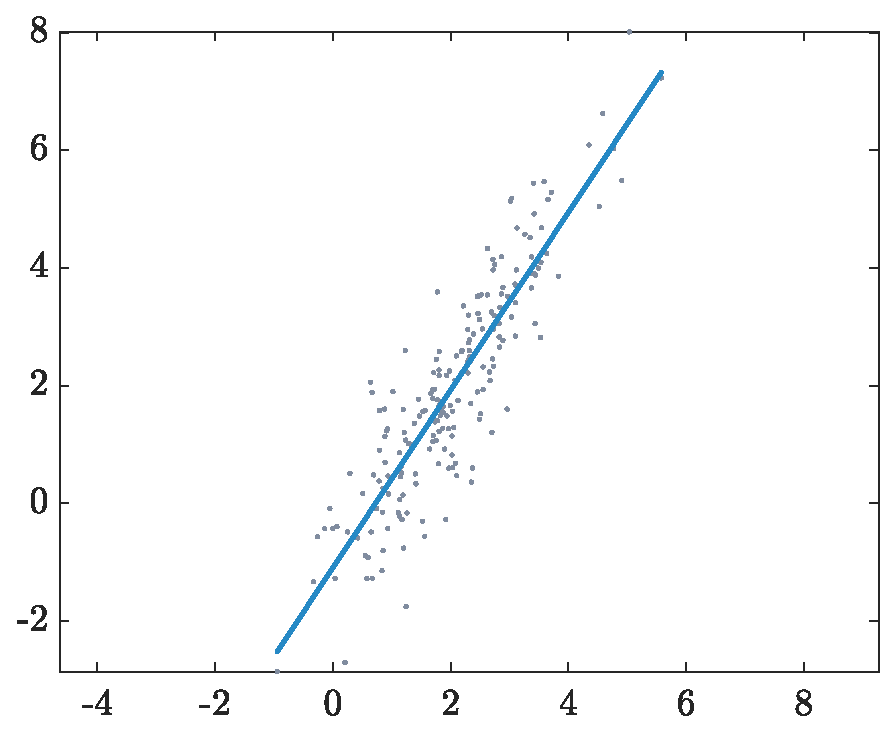
\includegraphics[width=6cm]{LS-linear-basis-functions.eps}
\caption{Linear basis function LS regression.}
\label{fig:LS-linear-basis}
\end{figure}

\begin{figure}[H]
\centering\includegraphics[width=6cm]{LS-nonlinear-basis-functions.eps}
\caption{Non-linear (quadratic) basis function LS regression.}
\label{fig:LS-linear-basis}
\end{figure}



\section{Connection to Singular Value Decomposition}




\section{Moore-Penrose pseudo-inverse}


\newpage


\thebibliography{}



\bibitem{Strang} G. Strang, \textit{Introduction to Linear Algebra}, Fifth Edition, 2016

\bibitem{Bishop} C. M. Bishop, \textit{Pattern Recognition and Machine Learning}, 2006

\bibitem{Kutz} N. Kutz, \textit{Data Driven Discovery of Dynamical Systems and PDEs}, an online lecture 

\bibitem{Tibishrani} T. Hastie, R. Tibshirani, J. Friedman, \textit{Elements of Statistical Learning, Data Mining, Inference, and Prediction}, Second Edition, 2008

 \label{bib:pope}


\end{document}
